\documentclass{article}
\usepackage[preprint]{corl_2026}
\usepackage{graphicx,booktabs,amsmath,amssymb}
\title{Spatial Instruction Following in World--Action Models}
\author{Anonymous Authors}
\begin{document}
\maketitle
\begin{abstract}
When a robot succeeds at \emph{right of the bowl} but fails at \emph{left of the bowl}, does it misunderstand the instruction, or is one placement harder in that scene? We study Cosmos 3 Nano and DreamZero in a simulated cube-placement task. For each model, 108 trials cross two commands with two object layouts while keeping the model, robot, cameras and controller fixed. Mirroring the object positions changes DreamZero's task completion from 13/54 to 50/54 trials. Most of its original-layout failures occur at pickup or transport. Nano remains highly successful, but the side on which it places the cube farther beyond the bowl reverses. Its final cube--bowl positions follow the requested LEFT/RIGHT ordering in every matched pair in both layouts. These results distinguish response to an instruction from successful execution: scene layout can change task performance substantially even when a model responds to the directional words.
\end{abstract}
\keywords{World--action models, spatial instructions, robot manipulation}

\section{Introduction}
A robot asked to place a cube on either side of a bowl must do more than recognize \emph{left} and \emph{right}. It must also grasp the cube, transport it and release it in the requested region. An instruction can redirect the robot in the correct direction while the final placement still fails. A difference in LEFT and RIGHT success rates therefore leaves an important question unanswered: did the instruction fail to influence the policy, or did the resulting motion fail to complete the task?

This distinction matters for world--action models, which connect visual world modeling with robot control. DreamZero jointly models future video and actions, while the Cosmos 3 family supports both world modeling and policy generation~\citep{ye2026dreamzero,nvidia2026cosmos3}. Their ability to follow a spatial instruction must still be established through the robot's behavior. Existing world-model benchmarks assess functional utility alongside visual quality~\citep{shang2026worldarena}. We examine how to interpret performance on the executed manipulation task.

Our experiment mirrors the positions of movable objects while keeping the policy and commands fixed. In each layout, we compare LEFT and RIGHT trials that begin from the same physical state. We separately measure how the command changes the final cube--bowl relation, how far the cube finishes on the requested side, and whether the placement succeeds. DreamZero's completion rate changes substantially with layout; Nano's achieved placement changes even when completion remains high. The contribution is a controlled demonstration that task success and directional response can support different conclusions about the same world--action model.

\section{Experimental Setup}
\paragraph{Task and models.}
We evaluate Cosmos 3 Nano and DreamZero on a Rubik's-cube placement task in the DROID/RoboLab simulator. The command is \emph{Put the Rubik's cube to the [left/right] of the bowl}. It remains fixed throughout each execution, which permits at most 450 actions. The robot receives no intermediate hints.

\paragraph{Scene intervention and repeated trials.}
The reflected layout mirrors the centers of all movable objects across the robot's forward midline. The robot, cameras, fixed scene geometry and controller remain unchanged. LEFT continues to mean the robot's left in both layouts (Figure~\ref{fig:design}).

\begin{figure}[t]
\centering
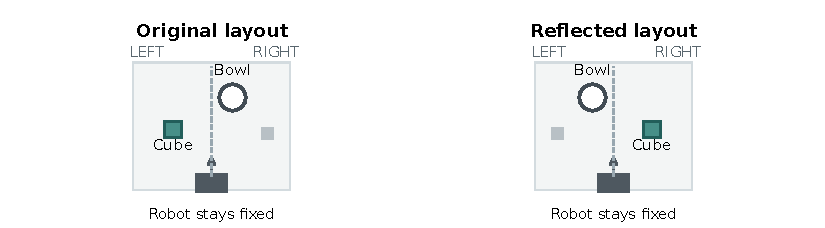
\includegraphics[width=\linewidth]{figures/reflection_design.pdf}
\caption{\textbf{Change the layout, repeat the commands.} Both LEFT and RIGHT instructions are tested in each arrangement. Movable objects are reflected, while the robot and cameras remain fixed. The diagram is schematic; it does not show measured coordinates or a recorded trajectory.}
\label{fig:design}
\end{figure}

Each model has 27 matched trial blocks. A block contains four executions: both commands in the original layout and both in the reflected layout, giving 108 trials per model. The starting physical state is identical across repeats within each layout. These are two fixed layouts, not 27 different scenes. Nano uses matched policy-sampling seeds across conditions. DreamZero's inference configuration fixes its noise seed, so its repeats are not independent draws of model noise. We report the models separately.

\paragraph{Measurements.}
Let $y$ denote the final cube--bowl lateral offset, positive to the robot's left. For a matched pair of commands, the \emph{instruction response}
\begin{equation}
R=y_{\mathrm{LEFT}}-y_{\mathrm{RIGHT}}
\end{equation}
is positive when asking for LEFT places the cube farther left relative to the bowl than asking for RIGHT. Because the bowl is movable, this measures a change in their spatial relation, not the separation of two absolute cube endpoints.

The \emph{placement depth} is the final offset toward the requested side: $y_{\mathrm{LEFT}}$ for LEFT and $-y_{\mathrm{RIGHT}}$ for RIGHT. A larger positive depth means the cube finishes farther past the bowl on that side. We compare the two requests using
\begin{equation}
G=(-y_{\mathrm{RIGHT}})-y_{\mathrm{LEFT}}.
\end{equation}
Positive $G$ favors rightward placement; negative $G$ favors leftward placement. We measure its change between layouts within each trial block. Depth is a final position, not distance traveled from the start.

Task success requires the cube to be released within 45 degrees of the requested left/right direction from the bowl. A favorable lateral offset alone need not satisfy this rule. We use the same rule in both layouts and calculate both position measures over all trials, including failed placements. All measurements concern executed behavior recorded by the simulator. Nano's confidence intervals use 20,000 bootstrap resamples of complete trial blocks, keeping all four conditions together; DreamZero's repeated-run results are reported descriptively.

\section{Results}
\begin{table}[t]
\centering
\caption{\textbf{Task completion and instruction response describe different aspects of behavior.} Success counts have 27 trials each. $R$ is the mean LEFT-minus-RIGHT difference in final cube--bowl offsets. $G$ compares achieved placement depth, with positive values favoring RIGHT requests.}
\label{tab:results}
\begin{tabular}{llrrrr}
\toprule
Model & Layout & \shortstack{LEFT\\success} & \shortstack{RIGHT\\success} & \shortstack{$R$\\(cm)} & \shortstack{$G$\\(cm)}\\
\midrule
Nano & Original & 26/27 & 26/27 & 44.8 & $+14.8$\\
 & Reflected & 27/27 & 23/27 & 45.3 & $-10.0$\\
DreamZero & Original & 5/27 & 8/27 & 12.2 & $+2.3$\\
 & Reflected & 25/27 & 25/27 & 37.6 & $-11.8$\\
\bottomrule
\end{tabular}
\end{table}

\paragraph{Layout strongly changes DreamZero's completion rate.}
DreamZero succeeds in 5/27 LEFT trials and 8/27 RIGHT trials in the original scene, compared with 25/27 in each direction after reflection (Table~\ref{tab:results}). Combined across commands, completion rises from 13/54 to 50/54 with the same checkpoint, wording and controller. Poor performance in the original scene is therefore insufficient evidence that the direction words were ignored or misunderstood.

\paragraph{High success can hide changes in achieved placement.}
Nano completes 26/27 trials for each command in the original layout. Yet its rightward placement depth exceeds its leftward depth by 14.8\,cm. After reflection, LEFT requests place the cube 10.0\,cm farther past the bowl than RIGHT requests. The mean within-block change in $G$ is $-24.8$\,cm. DreamZero's corresponding contrast changes from $+2.3$ to $-11.8$\,cm, a change of $-14.1$\,cm. Figure~\ref{fig:placement} contrasts these shifts with completion rates.

\begin{figure}[t]
\centering
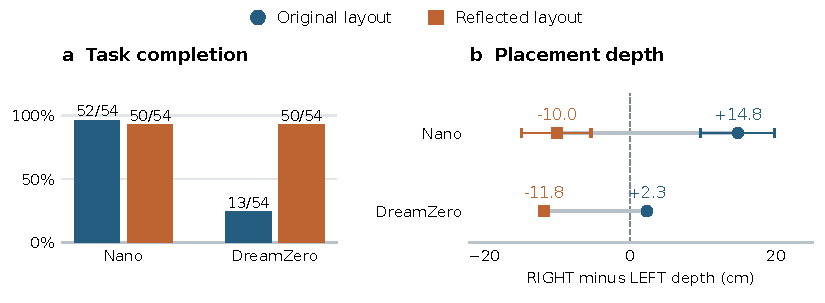
\includegraphics[width=\linewidth]{figures/reflection_results.pdf}
\caption{\textbf{The same intervention affects the models differently.} Left: successful trials across both commands, out of 54 per layout. Right: mean RIGHT-minus-LEFT placement depth $G$. Nano has 95\% intervals over matched sampling-seed blocks; DreamZero is shown descriptively because its noise seed is fixed. The mean depth difference changes sign in both models.}
\label{fig:placement}
\end{figure}

\paragraph{Most original-layout DreamZero failures occur before placement.}
Of its 41 unsuccessful trials, the recorded checks classify 26 as pickup failures, 14 as transport failures and one as wrong-side placement. These categories describe execution stages, rather than what the model understood. They show why the overall failure count cannot be treated as a count of directional-language errors.

\paragraph{Instruction response and placement depth need not change together.}
Nano's final cube--bowl offsets follow the command's directional ordering in all 27 pairs in each layout; DreamZero does so in 26/27 original-layout pairs and 27/27 reflected-layout pairs. Nano's mean response $R$ is 44.8\,cm before reflection and 45.3\,cm afterward. Its estimated change in response is much smaller than the 24.8\,cm change in relative placement depth. This does not establish exact invariance. DreamZero's response increases from 12.2 to 37.6\,cm: layout can affect both the response to a command and the success of its execution.

Nano's mean change in $G$ has a 95\% interval of $[-32.4,-17.3]$\,cm. This summarizes variation across sampling-seed blocks in the two tested layouts, not generalization to new scenes. We make no inference over independent model-noise samples for DreamZero.

\section{Discussion and Limitations}
The results separate three questions: does language change the cube--bowl relation in the requested direction, how far does the achieved placement extend toward the goal, and does the full manipulation succeed? Nano shows why continuous position matters near a success ceiling. DreamZero shows how much completion can change with another object arrangement. In both cases, the scene is part of the explanation of the score.

For world--action model evaluation, a useful comparison is to repeat opposing commands from the same state, then repeat that comparison in a controlled alternative layout. Final object positions should accompany completion rates. A benchmark using one arrangement can otherwise turn a scene-specific execution difficulty into an apparent general limitation of spatial instruction following.

The study covers two checkpoints, one simulated task and two fixed layouts. Reflection changes objects' positions relative to the robot and cameras; it does not isolate reachability, visibility, grasp geometry or a model component. The commands test a familiar LEFT/RIGHT contrast rather than general language comprehension. We do not compare against policies without world modeling, so the results do not identify a causal benefit or disadvantage of world modeling. Executed outcomes also do not establish the accuracy of generated future videos. Comparing predicted and actual object positions at matching times would address that separate question.

\section{Conclusion}
Changing the object layout substantially changes spatial task performance without changing the evaluated models or their commands. Measuring instruction response, placement depth and completion separately shows what a success rate alone misses. This distinction is necessary when using manipulation benchmarks to assess spatial instruction following in world--action models.

\bibliography{references}
\end{document}
